\documentclass[]{beamer}

\usepackage[utf8]{inputenc}
\usepackage{lmodern}
\usepackage{beamerthemesplit} 
\usepackage{pstricks}
\usepackage{pst-node}
\usepackage{graphicx}

\title[Semi-Lagrangian scheme multidimensional Black-Scholes]{Semi-Lagrangian scheme for multidimensional Black-Scholes PDE}
\author[Quoc Cuong NGUYEN and Chi Thanh NGUYEN]{NGUYEN Quoc Cuong \and NGUYEN Chi Thanh}
\institute[PDE - M2MO]{\large Profs : Y. Achdou - O. Bokanowski}
\date{05 Mai 2014}

\begin{document}
\footnotesize
\begin{frame}[plain]
\titlepage
\end{frame}

\begin{frame}
\tableofcontents
\end{frame}

\section{Black-Scholes Multidimensional - basket option}
\subsection{The model}
\begin{frame}
\frametitle{Black-Scholes model}
\small
Asset dynamic
\[
dS_t = \textbf{diag}(S_t) [\mu_t dt  +  \beta dW_t]
\]
Risk neutral probability
\[
\left. \frac{d \mathbb{P}^* }{d\mathbb{P}}\right|_{\mathcal{F}_T} 
= \text{exp}\{ - \int_0^t \theta_u dW_u - \frac{1}{2} \int_0^t |\theta_u|^2 du \}
\]
Pricing formula
\[
P_t = V_t = e^{ -\int_t^T r_u du } \mathbb{E}^* [\varphi(S_T) | \mathcal{F}_t]
\hspace{1cm}
P_T = V_T = \varphi(S_T)
\]
Possibilities
\begin{itemize}
 \item interest rate dependent to time
 \item local volatility
\end{itemize}
\end{frame}
%%%%%%%%%%%%%%%%%%%%%%%%%%%%%%%%
\subsection{PDE pricing}
\begin{frame}
\frametitle{PDE Black-Scholes}
Feymann-Kac formula with condition $r_t$ is bounded
\[
v(t,x) = e^{ -\int_t^T r(u) du } \mathbb{E}^* [\varphi(S_T) | S_t = x]
\]
equivalent to
\[
\partial_t v(t,x) + \mathcal{A} v(t,x) - r(t)v(t,x) = 0 
\hspace{1cm}
v(T,x) = \varphi(x)
\]
Resolution methods :
\begin{itemize}
 \item analytical approach : Finite Difference (Taylor expansion, implicite/explicite)   
 \item probabilistic approach : Markov chain ( \textbf{H.J. Kushner} 1992 )
\end{itemize}
\end{frame}
%%%%%%%%%%%%%%%%%%%%%%%%%%%%%%%%
\subsection{Closed form for particular payoff}
\begin{frame}
\frametitle{Closed form for particular payoff (1/2)}
Variable change $w(T,y)=v(T,x)$ where $y=\sum \alpha_i x_i$ :
\[
\left\{
\begin{array}{ll}
\partial_t v +\frac{1}{2} \text{Tr}(\sigma \sigma^{t} \textbf{D}^2 v ) +rx .\triangledown v - r v =0 \\ \\
v(T,x) = \varphi(x) = (K-\sum \alpha_i x_i)
\end{array}
\right.
\]
\[\label{eq:diff_w}
\frac{\partial v}{\partial x_i}(t,x) = \alpha_i \frac{\partial w}{\partial y} (t,y)
\hspace{2cm}
\frac{\partial^2 v}{\partial x_ix_j}(t,x) = \alpha_i\alpha_j \frac{\partial^2 w}{\partial y^2} (t,y)
\]
\[
\text{Tr}(\sigma \sigma^{t}.\alpha\alpha^{t}) 
= \text{Tr}( \textbf{diag}(x) \beta\beta^{t} \textbf{diag}(x)^t.\alpha\alpha^{t})
= \sum_{i,j=1}^d \alpha_i\alpha_j x_i x_j <\beta_i , \beta_j>
\]
\end{frame}
%%%%%%%%%%%%%%%%%%%%%%%%%%%%%%%%
\begin{frame}
\frametitle{Closed form for particular payoff (2/2)}
Under condition $\beta\beta^{t} = \check{\sigma}^2 \textbf{J}$ this lead to equivalent unidimensional problem
\[
\longrightarrow\left\{
\begin{array}{ll}
\partial_t w +\frac{1}{2} \check{\sigma} y^2 \partial_{yy} w  +  r y \partial_{y} w - r w = 0 \\ \\
w(T,y) = (K-y)^+
\end{array}
\right.
\] 
Exact Black-Scholes formula
\[
w(t,y) =- y \mathcal{N}(-d_+) + e^{-r(T-t)} K \mathcal{N}(-d_-)
\]
\[
d\pm = \frac{ \text{log}(\frac{y}{K}) + (r \pm \frac{\check{\sigma}^2}{2} )(T-t) } {   \check{\sigma}  \sqrt{T-t} }
\]

\end{frame}
%%%%%%%%%%%%%%%%%%%%%%%%%%%%%%%%
\section{Approximation Order 1}
\subsection{Euler Approximation}
\begin{frame}
\frametitle{Euler Approximation}
Approximation of underlying asset  : 
\[
dS_t = \textbf{diag}(S_t) [\mu_t dt  +  \beta dW_t]
\]
Given a time discretization of interval $[0,T]$ 
\[0<t_1=h<\dots<t_n=nh<\dots<t_N=T\] \\
Euler Weak Approximation :
\[
Y^k_{n+1}=Y^k_n+ r hY^k_n  + Y^k_n\sum_{j=1}^d (\beta)^{k,j} (\Delta \hat{W})^j, \hspace{0.2cm} \forall n \in \{1,\dots,N\}
\]
where $\Delta \hat{W}^j$ could be 
\begin{itemize}
 \item Gaussian Increments $\Delta W \approx N(0,h)$
 \item A two-point distributed random variable with : $\mathbb{P}^*(\Delta\hat{W}^j=\pm \sqrt{h})=\frac{1}{2}$
\end{itemize}
\end{frame}
%%%%%%%%%%%%%%%%%%%%%%%%%%%%%%%%
%%%%%%%%%%%%%%%%%%%%%%%%%%%%%%%%
\subsection{Semi-Lagrangian}
\begin{frame}
\frametitle{Semi-Lagrangian d=1}
Unidimensional Euler Approximation + $\Delta \hat{W}$ two points distributed
\[\mathbb{E}^*[Y_{n+1}|Y_n=x] =\frac{1}{2}\left\lbrack x+rhx+\beta x
\sqrt{h}\right\rbrack +\frac{1}{2}\left\lbrack x+rhx-\beta x \sqrt{h} 
\right\rbrack\]
PDE's Pricing Formula for discounted porfolio $\tilde{v}$: 
\[\tilde{v}(t_{n},x)=\mathbb{E}^*\lbrack\tilde{v}(t_{n+1},X_{t_{n+1}})|X_{t_n}=x\rbrack\]
\[\longrightarrow \mathbb{E}^*\lbrack\tilde{v}(t_{n+1},Y_{n+1})|Y_{n}=x\rbrack 
= \sum_{\varepsilon=\pm 1}\frac{1}{2}\tilde{v}(t_{n+1},x+rhx+\varepsilon\beta x \sqrt{h})
\]
Approximate $\tilde{v}$ by : 
\[\tilde{u}(t_{n},x)= \frac{1}{2} \sum_{\varepsilon = \pm1} 
\left\{
\tilde{u}\left(t_{n+1},x + hb_k(x) + \varepsilon \sqrt{h} \sigma_k (x) \right)
\right\}\]
\end{frame}
%%%%%%%%%%%%%%%%%%%%%%%%%%%%%%%%
\begin{frame}
\frametitle{Semi-Lagrangian d greater than 1}
Generalization for superior dimension 
\[u(t_{n},x)= \frac{e^{-rh}}{2d} \sum_{\varepsilon = \pm1} \sum_{k=1}^d 
\left\{
u\left(	t_{n+1},x + hb_k(x) + \varepsilon \sqrt{h} \sqrt{d}  \sigma_k (x) \right)
\right\} \]
\[u(T,x) = v(T,x)= \varphi(T)
\]
\begin{itemize}
 \item d directions equally probable with probability = 1/d
 \item Interpolation necessary 
 \begin{itemize}
  \item $P_1: |[\psi ](x)-\psi(x)|\leq\Delta x^2 $ for any $C^2$ regular function $\psi$
  \item $Q_1: |[\psi ](x)-\psi(x)|\leq L\Delta x  $ for any Lipschitz-continous function $\psi$
 \end{itemize}

\end{itemize}
\end{frame}
%%%%%%%%%%%%%%%%%%%%%%%%%%%%%%%%
\subsection{Error Analysis}
\begin{frame}
\frametitle{Scheme Error}
Consistency error for P1 Interpolation type : 
\[ \frac{1}{h} |v^n(x) -(Sv^{n+1})(x)| \leq\  T(\frac{P\Delta x^2}{h}+Ch) \]
Thus, True Error : 
\[|u^n(x)-v^n(x)|  \leq T(\frac{P\Delta x^2}{h}+Ch)\]
\begin{itemize}
 \item C depends on : $||\textbf{D}^2_xv||_\infty $, $||\textbf{D}^3_xv||_\infty$, $||\textbf{D}^4_xv||_\infty $ and $sup_{t,x}||\partial_{tt}v(t,x)||$ 
 \item $\Delta x \approx h \longrightarrow$ : errors linear in h 
\end{itemize}
\end{frame}
%%%%%%%%%%%%%%%%%%%%%%%%%%%%%%%%
\section{Results from approximation order 1}
\subsection{Verification d=2 : Comparison with exact solution}
\begin{frame}
\frametitle{Comparison with exact solution}
%\begin{figure}[ht]
%\centering
%\subfigure[Profile View]{
\includegraphics[scale=0.3]{EDP_2dim_profile_view.eps}
%}
%\quad
%\subfigure[Level set $10^{-2}$]{
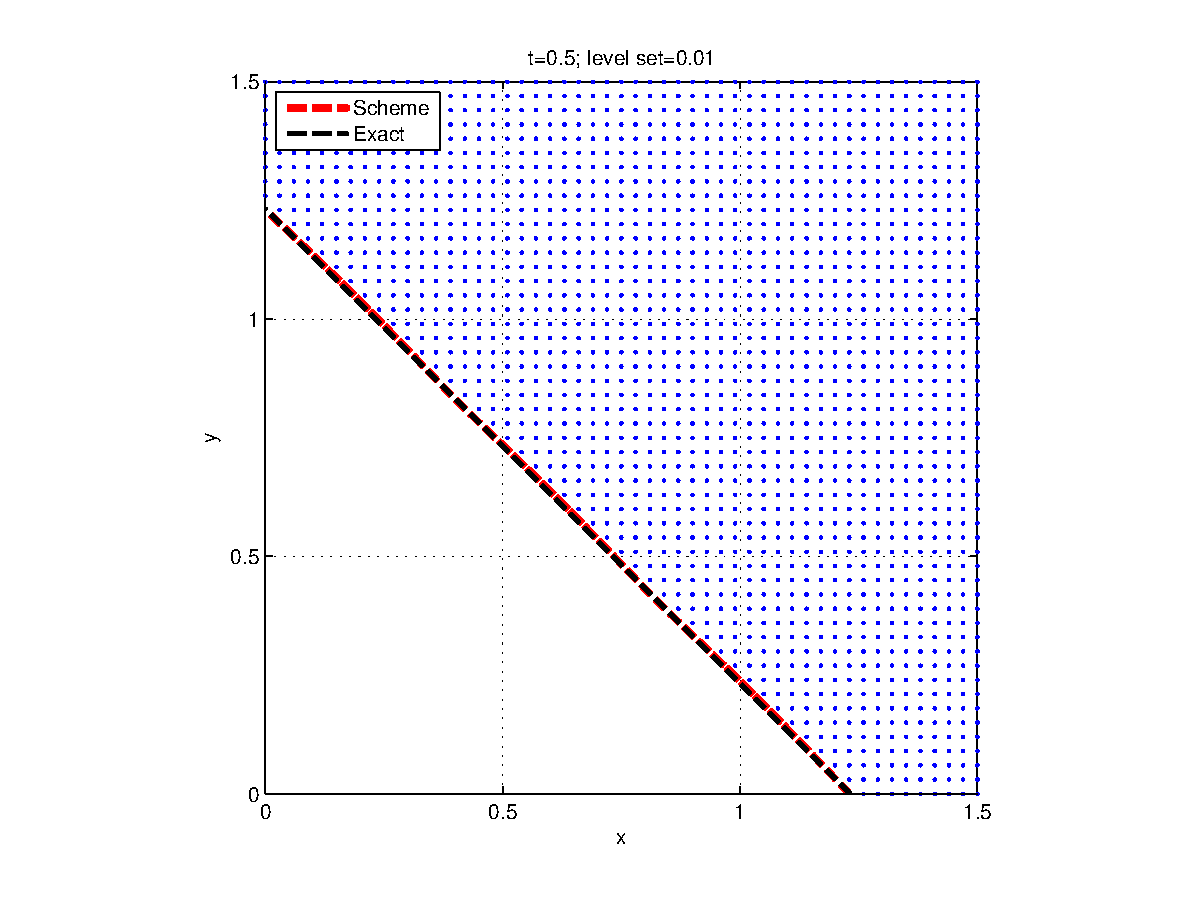
\includegraphics[scale=0.3]{EDP_isoline_lvlE-2.eps}
%}
%caption[Payoff ]{Payoff \hspace{0.1cm}$ y=x_1+x_2$}
%\end{figure}
\begin{center}
Payoff : $ (K-(S^1+S^2))^+$
\end{center}
\end{frame}
%%%%%%%%%%%%%%%%%%%%%%%%%%%%%%%%
\subsection{Verification d=2 : Error Linear Dependance}
\frametitle{Error Dependance}
\begin{frame}
\begin{center}
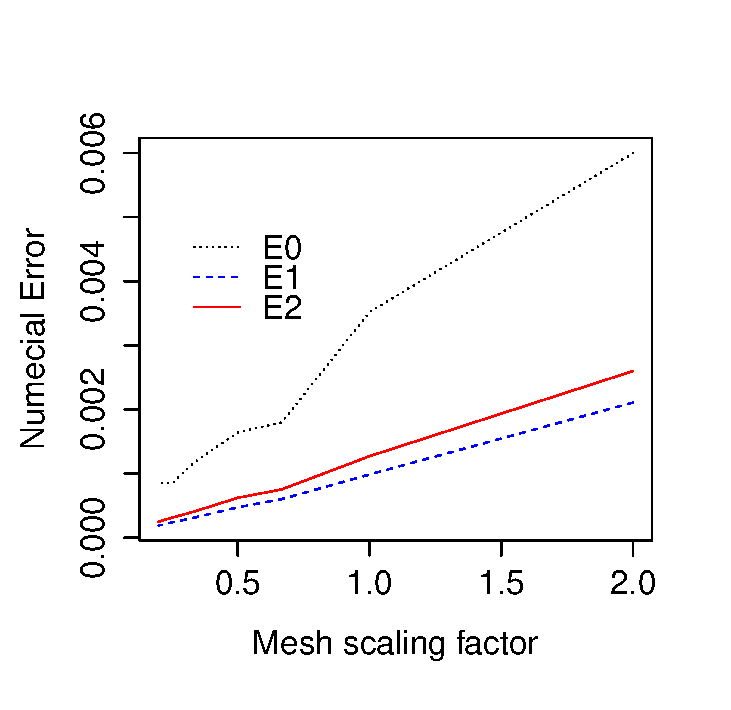
\includegraphics[scale=0.6,keepaspectratio=true]{linear_error}
\end{center}
\end{frame}
%%%%%%%%%%%%%%%%%%%%%%%%%%%%%%%%
\subsection{Other 2d-Payoff : Max \& Min Put}
\begin{frame}
\frametitle{Max-Put \& Min Put}
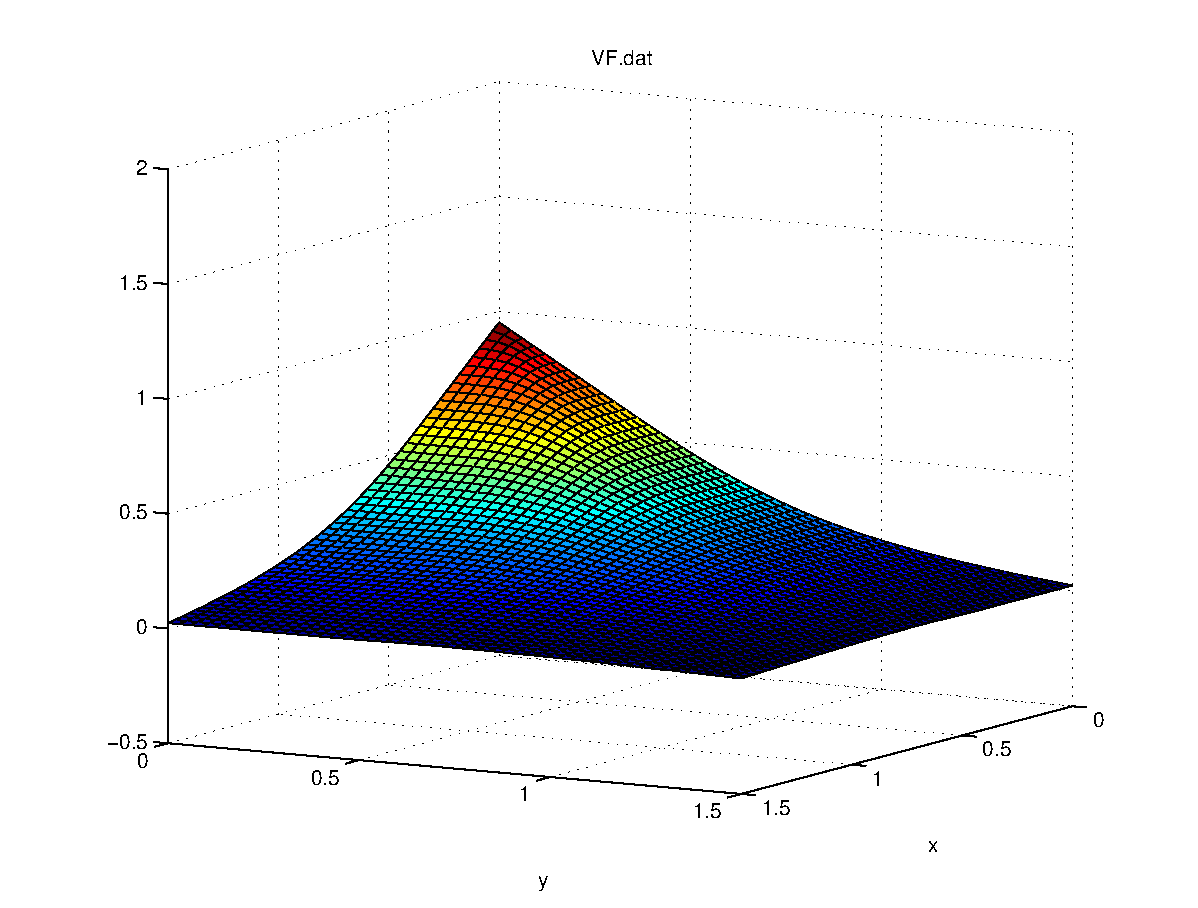
\includegraphics[scale=0.3]{put_max_2d.eps}
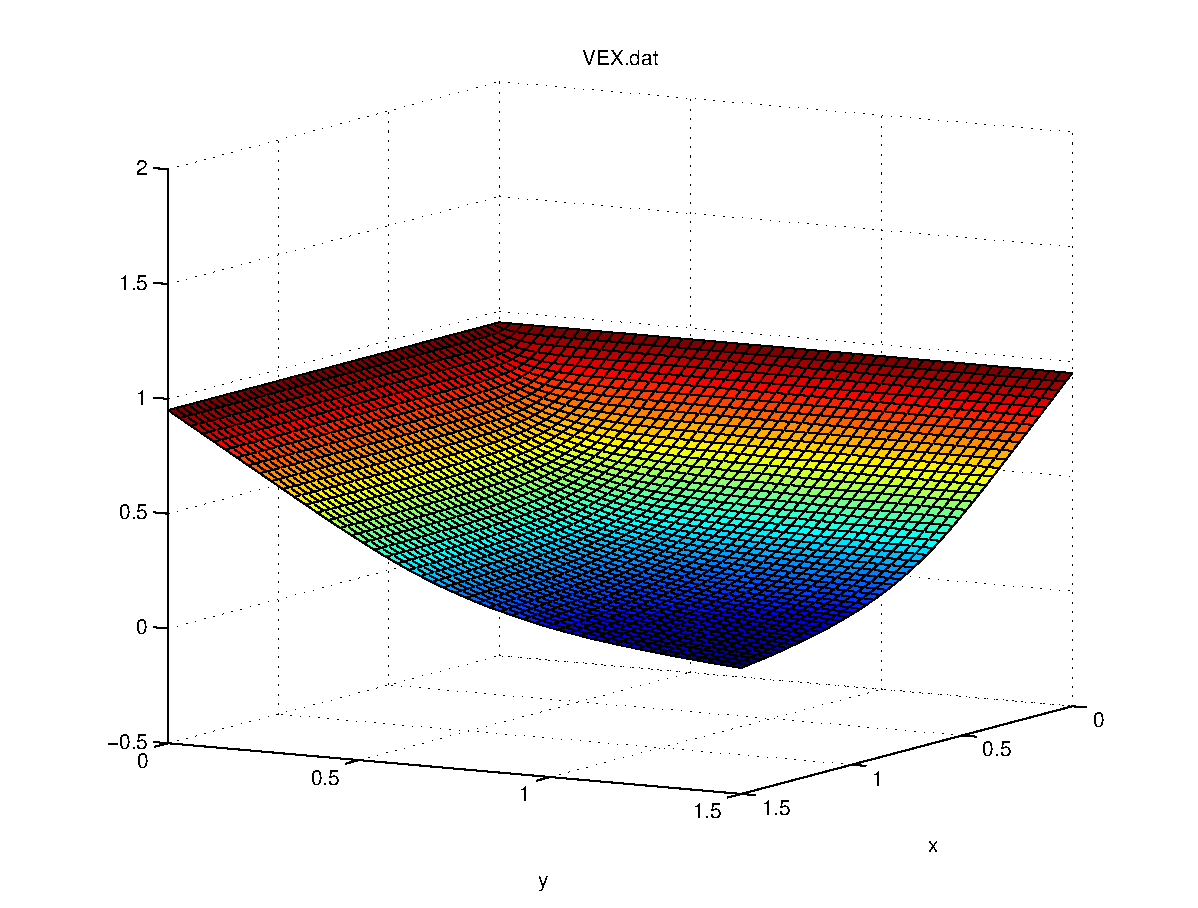
\includegraphics[scale=0.3]{put_min_2d.eps}
\end{frame}
%%%%%%%%%%%%%%%%%%%%%%%%%%%%%%%%
%%%%%%%%%%%%%%%%%%%%%%%%%%%%%%%%
\subsection{Higher Dimension}
\frametitle{High Dimension}
\begin{frame}
\frametitle{Higher Dimension}
\begin{center}
\begin{tabular}{l|c|c|c|c}
%%\hline
Dimension   &  2          & 3       & 4       & 5  \\
\hline\hline
Elapsed time(s)  &  0.00775807 & 0.10785 & 4.12525 & 182.404 \\
%\hline
\end{tabular}
\end{center}
\begin{itemize}
 \item Pre-compute interpolation takes a lot of memory 
 \item Without pre-compute, caculation takes lots of time
\end{itemize}

\end{frame}
%%%%%%%%%%%%%%%%%%%%%%%%%%%%%%%%
\section{Proposal order 2 Platen schemes}
\subsection{Platen Approximation}
\begin{frame}
\frametitle{Platen Approximation}
Platen Weak Approximation Scheme : 
\begin{equation*}
u_n(x) = \frac{e^{-rh}}{6d}\sum^d_{k=1} \left\lbrace u_{n+1}[Y^{-1}_k(x)] +  4u_{n+1}[Y^{(0)}_k(x)]+ u_{n+1}[Y^{+1}_k(x)] \right\rbrace
\end{equation*}
where 
\begin{equation*}
Y^{\varepsilon}_{k}(x) = x 
                     + (h + \frac{h^2r}{2}  ) rx
                     + \varepsilon \sqrt{3dh}(rh + 1 )  x*\beta_k
                     + \frac{h}{2}(-1 + \varepsilon^2 3d)x*\beta_k*\beta_k       
\end{equation*}
$*$ operator as $[a*b*c]_i = a_ib_ic_i$
\begin{itemize}
 \item Simple genalization from unidimensional : d directions uniformly distributed
 \item Three points distribution to approximate $\Delta W \approx N(0,h) $
 \[\mathbb{P}(\Delta\hat{W}=\pm \sqrt{3dh})=\frac{1}{6d} \hspace{2cm} \mathbb{P}(\Delta\hat{W}=0)=\frac{2}{3d} \]
\end{itemize}
\end{frame}
\subsection{Comparaison with Euler}
\begin{frame}
\frametitle{Comparaison with Euler}
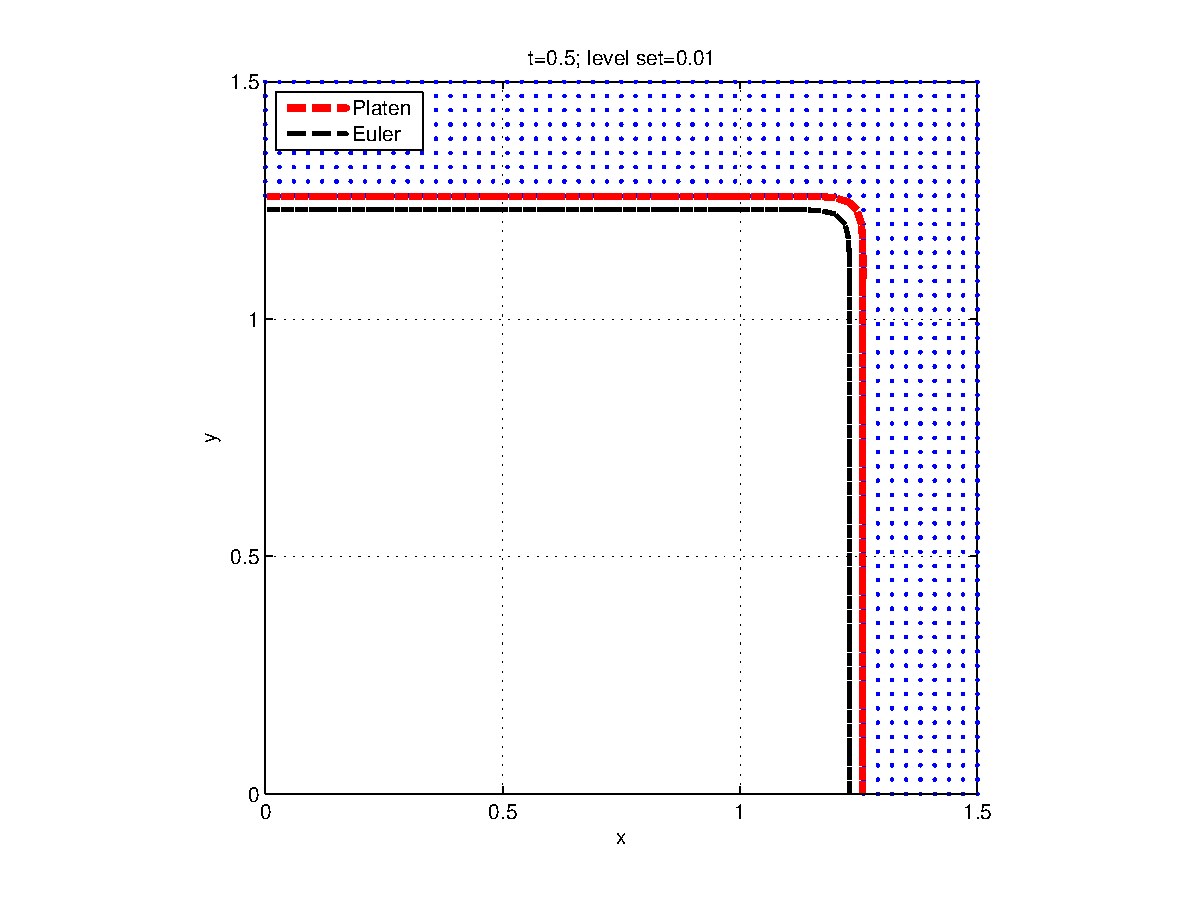
\includegraphics[scale=0.3]{put_max_vs.eps}
\includegraphics[scale=0.3]{put_weighted_vs.eps}
\end{frame}
\section{Conclusion}
\begin{frame}
\frametitle{Conclusion}
 \begin{itemize}
  \item PDE's Mutltidimensional Black-Scholes pricing option
  \item Closed form for particular payoff
  \item Library \textbf{HJB-Solver} coded in C++
  \item Semi-Lagragian 
  \begin{itemize}
   \item Euler Approximation
   \item Consistency, True Error Order 1
   \item Algorithm parallelizable
  \end{itemize}
\item Platen Approximation 
\begin{itemize}
 \item Simple Generalization : Results Order 1 $\longrightarrow$ Adjust points
 \item Multidimensional Approximation Formula  : more sophisticated
\end{itemize}

 \end{itemize}

\end{frame}
\section*{Apprendix}
\subsection*{Platen Weak Approximation d = 1}
\begin{frame}
The idea is to approximate the SDE verified by S unidimensional by the following scheme
\begin{equation*}
\begin{split}
Y_{n+1}=Y_n+&\frac{1}{2}(r\bar{\Upsilon}+rY_n)h+\frac{1}{4}(\beta\bar{\Upsilon}^+ + \beta\bar{\Upsilon}^-+2\beta Y_n)\Delta\hat{W}\\
&+\frac{1}{4}(\beta\bar{\Upsilon}^+ - \beta\bar{\Upsilon}^-)\left\lbrace(\Delta \hat{W})^2-h \right\rbrace h^{-1/2}\\
\end{split}
\end{equation*}
where 
\begin{equation*}
\left\lbrace
\begin{array}{l}
\bar{\Upsilon}=Y_n + rY_nh + \beta Y_n \Delta \hat{W}, \\
\bar{\Upsilon}^{\pm}=Y_n + rY_nh \pm \beta Y_n \sqrt{h}
\end{array}
\right.
\end{equation*}
$\Delta\hat{W}$ could be Gaussian or it could be three points distributed with :
\begin{equation*}
\mathbb{P}(\Delta\hat{W}=\pm \sqrt{3h})=\frac{1}{6} \hspace{2cm} \mathbb{P}(\Delta\hat{W}=0)=\frac{2}{3} 
\end{equation*}
The semi-Lagrangian version of Platen scheme will be : 
\begin{equation*}
u_n(x) = \frac{e^{-rh}}{3}\left\lbrace2u_{n+1}(Y^{(0)}(x))+ \frac{u_{n+1}(Y^{+}(x))}{2}+ \frac{u_{n+1}(Y^{-}(x))}{2}\right\rbrace
\end{equation*}
\end{frame}
\subsection*{Platen Weak Approximation d greater than 1}
\begin{frame}
\scriptsize
The vector form of multidimentional approximation is 
\begin{equation*}
\begin{split}
 &Y_{n+1} = Y_{n} + 
	  \frac{1}{2}( r\bar{\Upsilon}  + rY_n)h\\
         &+\sum^d_{j=1}\frac{1}{4}  \left\{
                           \left[  \sigma_j(\bar{R}^j_+ )  +  \sigma_j(\bar{R}^j_- )  + 2\sigma_j(Y_n)  \right]\Delta \hat{W}^j 
         +\sum^d_{r\neq j} \left[  \sigma_j(\bar{U}^r_+ )  +  \sigma_j(\bar{U}^r_- )  - 2\sigma_j(Y_n)  \right]\Delta \hat{W}^j 
                       \right\}  \\
	  &+\sum^d_{j=1}\frac{1}{4\sqrt{h} } \left\{
			    \left[  \sigma_j(\bar{R}^j_+ )  -  \sigma_j(\bar{R}^j_- )  \right] \left\{ (\Delta \hat{W}^j)^2 - h \right\} \right.\\
         &+\left.\sum^d_{r\neq j} \left[  \sigma_j(\bar{U}^r_+ )  -  \sigma_j(\bar{U}^r_- )  \right] \left\{ \Delta\hat{W}^r\Delta\hat{W}^j + V_{r,j} \right\}
                       \right\}
\end{split}
\end{equation*}
Where 
\begin{equation*}
\begin{array}{ll}
\bar{\Upsilon}=Y_n + rY_nh + \sum^d_{j=1} \sigma_j(Y_n) \Delta \hat{W}^j \\
\bar{R}^j_{\pm}=Y_n + rY_nh \pm \sigma_j (Y_n) \sqrt{h}  \\
\bar{U}^j_{\pm}=Y_n  \pm \sigma_j (Y_n) \sqrt{h}  \\
\end{array}
\hspace{0.5cm}
\begin{array}{ll}
\Delta \hat{W}^j \in \left\{ (-\sqrt{3h},\frac{1}{6}),(0,\frac{2}{3}),(\sqrt{3h},\frac{1}{6})   \right\} \\ 
V_{r,j} \in  \left\{ (-h,\frac{1}{2}),(h,\frac{1}{2}))   \right\}, \hspace{0.5cm} r < j \\  
V_{j,j} = -h  \\
V_{r,j} = -V_{j,r} , \hspace{2.5cm} r > j 
\end{array}
\end{equation*}


and

\end{frame}
\end{document}
